\section{Análise descritiva e agrupamento exploratório das formas}
\label{sec:analysisforms}

Esta etapa executa uma análise empírica dos registros já selecionados, distinta dos cenários prospectivos de amostragem. Seu objetivo é descrever a composição documental e explorar similaridades gráficas entre expressões, sem inferir origem, transmissão, prevalência populacional ou sucessão necessária de formas. Não foi treinado classificador supervisionado nem estimada capacidade de detectar novas ocorrências em acervos.

\subsection{Composição dos inventários e distribuição temporal}
A Figura~\ref{fig:composition} distingue o núcleo da seleção por quota. O primeiro contém \CoreRubrics{} rubricas e \CoreMimetic{} representações miméticas ou marcadores digitais; a segunda reúne 112 vínculos lexicais, 18 rubricas e cinco grafias miméticas. São inventários com funções e sobreposições diferentes. As barras descrevem os registros selecionados, não a proporção dessas práticas na sociedade.

\begin{figure}[htbp]
\centering\begin{minipage}{\textwidth}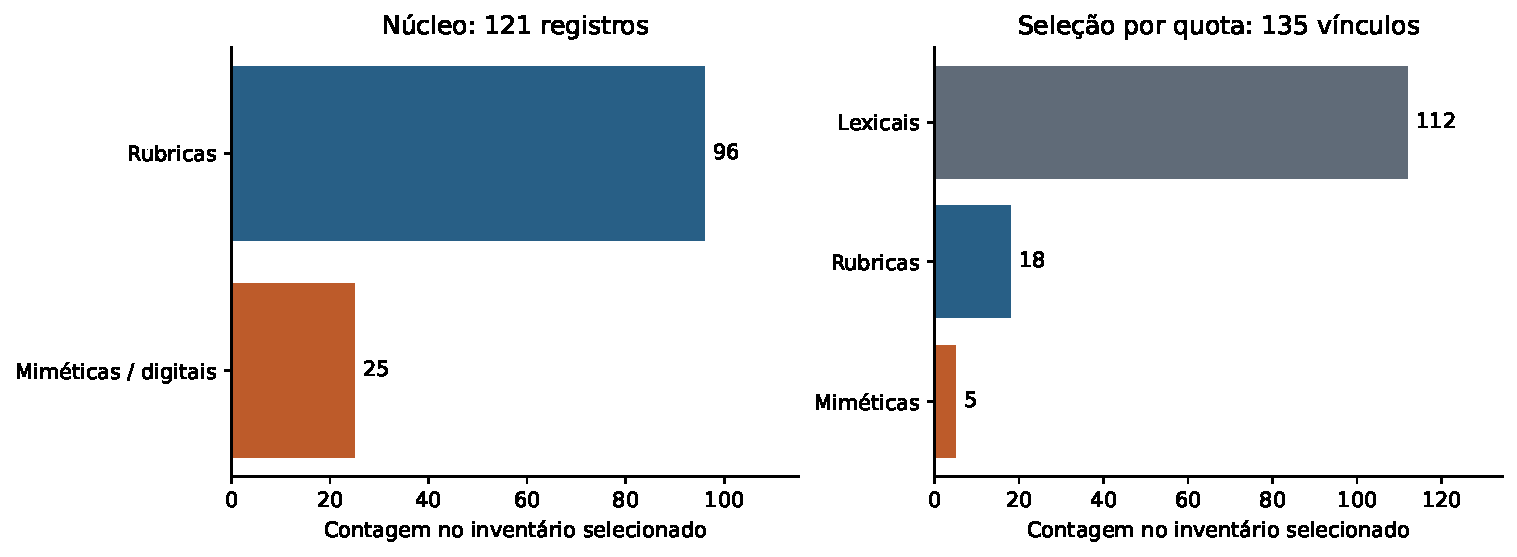
\includegraphics[width=\linewidth]{figures/analysis_composition.pdf}\end{minipage}
\caption{Composição dos dois inventários. Fonte: elaboração a partir dos CSV públicos. Os painéis não se somam como documentos independentes.}\label{fig:composition}
\end{figure}

A Figura~\ref{fig:decades} distribui o núcleo por década e categoria. Os dez registros por década entre 1900 e 2009 decorrem da estratégia de cobertura anual, com um testemunho por ano, e não de estabilidade histórica na frequência do riso. A década de 1890 não tem registro nesse núcleo, embora o levantamento complementar contenha documentos desse período. Não se interpola a lacuna nem se interpreta a altura das barras como intensidade de uso. Os documentos anteriores a 1872, presentes nos inventários complementares desde 1645, não integram esse gráfico do núcleo.

\begin{figure}[htbp]
\centering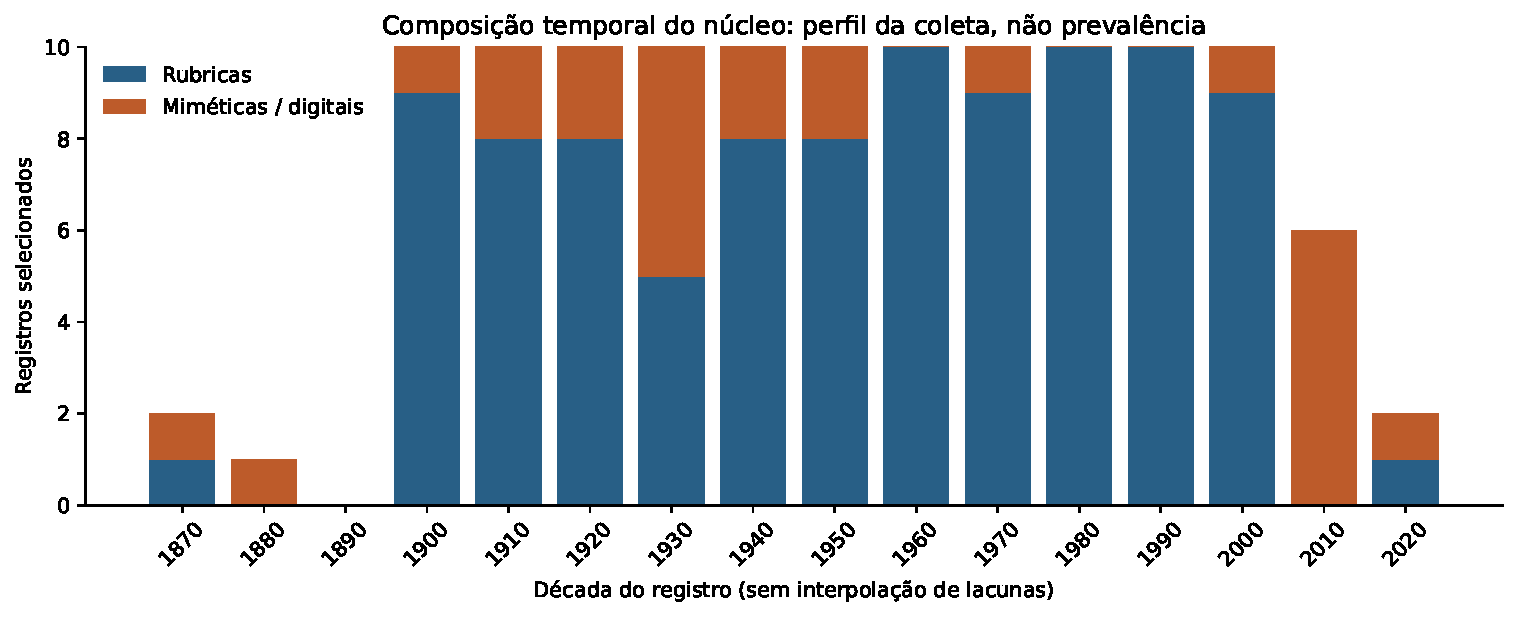
\includegraphics[width=\textwidth]{figures/analysis_decades.pdf}
\caption{Registros do núcleo por década. A distribuição é condicionada pelo protocolo de seleção; zero significa ausência de registro no inventário, não ausência histórica.}\label{fig:decades}
\end{figure}

A Figura~\ref{fig:all-decades} considera os quatro inventários positivos, com \EvidenceSources{} identificadores de fonte de \SelectedMinYear{} a \SelectedMaxYear{}, incluindo registros lexicais, lexicográficos, rubricas e grafias miméticas. O agrupamento por identificador evita somar vínculos repetidos; verificou-se que as datas atribuídas a um mesmo identificador são consistentes entre os inventários. O gráfico torna visível a extensão anterior a 1900, mas as diferenças entre décadas continuam dependentes da busca e da disponibilidade, sem estimar intensidade de uso ou representar independência histórica entre fontes.

\begin{figure}[htbp]
\centering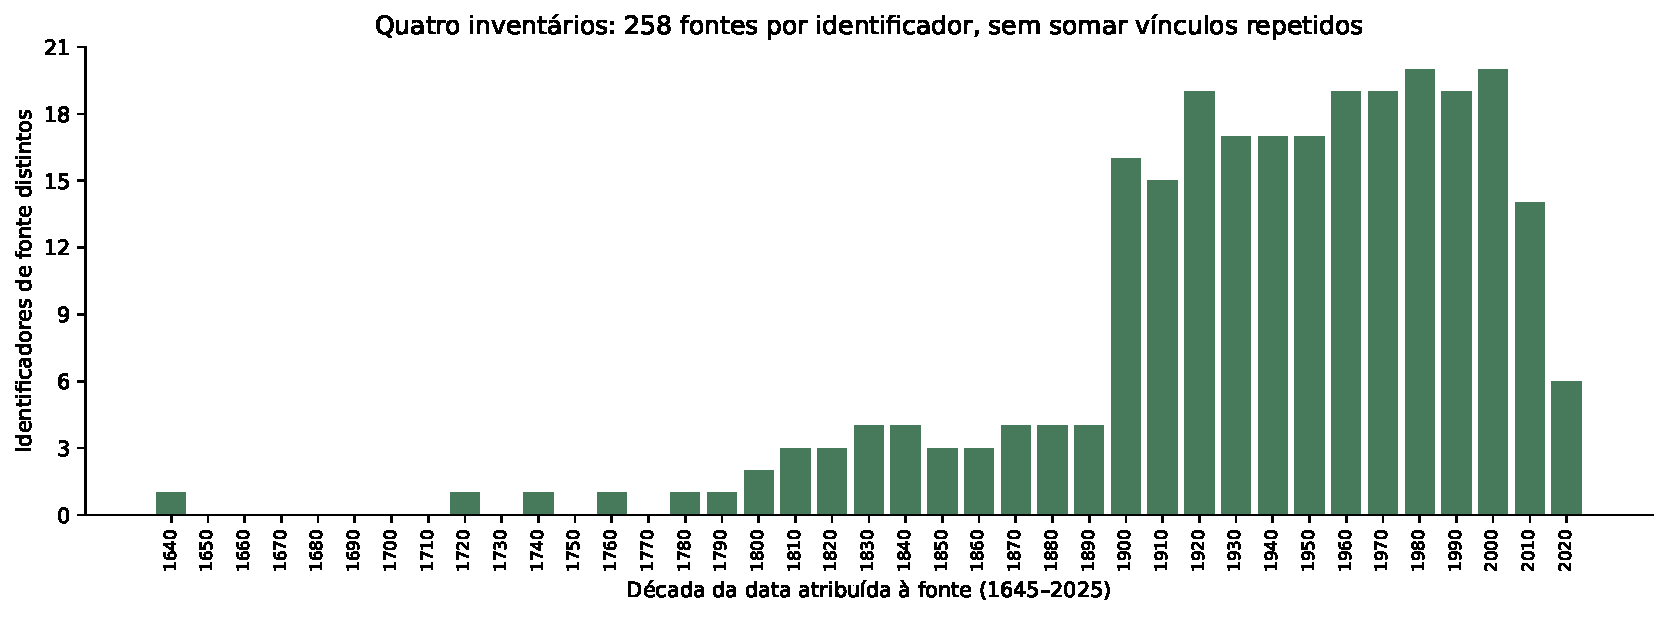
\includegraphics[width=\textwidth]{figures/analysis_all_decades.pdf}
\caption{Fontes por identificador e década nos quatro inventários positivos. A data é a atribuída ao registro, com as ressalvas de edição, interação ou captura publicadas nos CSV. Barras nulas indicam falta de fonte selecionada nesse conjunto.}\label{fig:all-decades}
\end{figure}

\subsection{Unidades, normalização e prevenção de circularidade}
O agrupamento restringe-se aos \CoreMimetic{} registros classificados como representações miméticas ou marcadores digitais. A coluna \texttt{form} descreve as sequências selecionadas, sem constituir transcrição exaustiva de todos os usos em cada documento. Um registro de chat reúne duas variantes separadas por barra; sua separação produz \AnalysisVariants{} vínculos de forma, sem criar novo documento. Após normalização, há \AnalysisForms{} sequências distintas. Cada sequência recebe peso igual, evitando que a repetição editorial de uma mesma grafia domine os grupos. Os vínculos com os registros originais são preservados.

A normalização aplica \textit{casefold}, decomposição Unicode NFKD e retenção apenas de letras. Assim, retiram-se acentos, espaços e pontuação para a comparação, mas a transcrição original permanece no CSV. Não se convertem letras em fonemas, não se substitui \forma{quiá} por \forma{quá} e não se iguala \forma{cá} a \forma{k}. O comprimento e a repetição das sequências são mantidos e podem influenciar as distâncias. Essas decisões definem um experimento sobre grafia normalizada, não sobre equivalência acústica ou interpretação pragmática.

Ano, país, suporte, acervo, nível de evidência e categoria documental não são variáveis do agrupamento. As categorias anteriores delimitam o subconjunto elegível, mas não são fornecidas como rótulos para formar grupos. As datas aparecem apenas depois, na descrição dos registros vinculados. A análise é condicionada à seleção documental e à normalização; não constitui validação independente da taxonomia usada para selecionar os 25 registros.

\subsection{Métodos e diagnósticos executados}
Compararam-se duas representações. No agrupamento hierárquico, a distância entre sequências é a distância de Levenshtein dividida pelo maior comprimento do par. A ligação média agrega as distâncias entre membros dos grupos; a ligação completa é usada como análise de sensibilidade \cite{scipyHierarchy2026}. No K-means, as variáveis são frequências TF-IDF de n-gramas de um a três caracteres, normalizadas em L2. Fixaram-se semente 0, 50 inicializações e limite de 300 iterações \cite{sklearnClustering2026}.

Para ambos, exploraram-se cortes de dois a seis grupos. Selecionou-se, dentro dessa grade, o maior coeficiente de silhueta, preferindo menor número de grupos em caso de empate exato. No método hierárquico, a silhueta usa a matriz de edição; no K-means, usa distância do cosseno no espaço TF-IDF, embora a otimização do K-means minimize distâncias euclidianas quadráticas. Portanto, os valores dos dois métodos não são comparados como uma escala comum para escolher um vencedor. A escolha interna na mesma grade e no mesmo conjunto é exploratória, sem teste externo de generalização.

Para o K-means, repetiram-se 20 inicializações isoladas, sementes 0 a 19, comparando cada partição à referência com 50 inicializações pelo índice de Rand ajustado (ARI). Avaliou-se ainda a troca de n-gramas 1--3 por 1--2. Para o hierárquico, compararam-se ligação média e completa no mesmo corte. O ARI também compara as partições escolhidas pelos dois métodos, independentemente dos números atribuídos aos grupos \cite{sklearnARI2026}. Esses diagnósticos medem sensibilidade computacional; não são intervalos de confiança, validação histórica ou confiabilidade de anotadores.

\subsection{Resultados e interpretação dos agrupamentos}
No hierárquico, o maior valor da grade foi obtido em \HierK{} grupos, com silhueta \HierSil{}. A solução em cinco grupos obteve 0,413, muito próxima da solução em quatro (diferença aproximada de 0,002). Não se apresenta, portanto, o corte em quatro como uma taxonomia definitiva. No K-means, a maior silhueta foi \KmeansSil{}, com \KmeansK{} grupos. Como seis é o limite superior da grade testada, o resultado não estabelece um ótimo global de número de grupos. O ARI entre as duas soluções selecionadas foi \MethodsARI{}.

No corte hierárquico em quatro, as variantes de \forma{ah/ha/he} ficam reunidas; outro grupo contém sequências de \forma{cá}, \forma{quá} e \forma{quiá}; as cadeias de \forma{k} formam um terceiro grupo; e \forma{rs} fica isolada. O K-means em seis separa \forma{cá} e \forma{hehehe} dos respectivos conjuntos maiores. A Tabela~\ref{tab:form-clusters} permite verificar a associação de cada sequência. Grupos unitários refletem a pequena amostra de formas e a parametrização; não comprovam categorias naturais da língua.

\begin{figure}[htbp]
\centering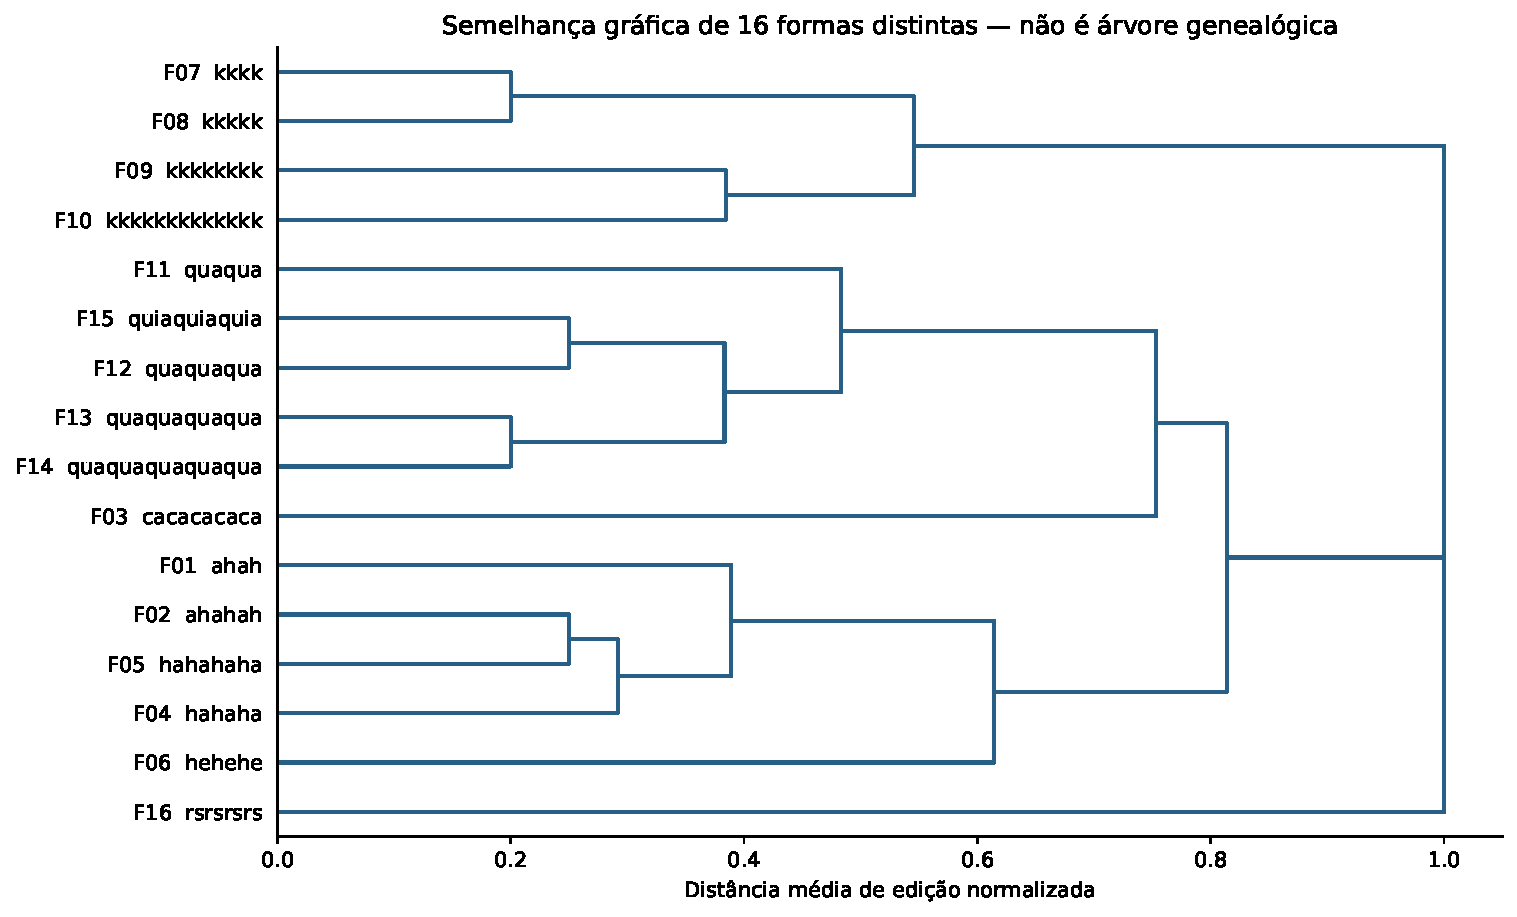
\includegraphics[width=\textwidth]{figures/analysis_dendrogram.pdf}
\caption{Dendrograma de ligação média sobre distância de edição normalizada. Os ramos representam operações de agrupamento computacional, sem direção temporal ou interpretação genealógica.}\label{fig:dendrogram}
\end{figure}

O agrupamento das cadeias de \forma{k} se manteve nas soluções selecionadas. Entretanto, a análise não colocou \forma{kkkk} no mesmo grupo de \forma{quiá} nesses dois cortes. Esse resultado é específico das variáveis e distâncias adotadas: não demonstra independência histórica, assim como uma proximidade gráfica não demonstraria filiação. As letras compartilhadas e o tamanho das sequências explicam parte das afinidades observadas, sem modelar processos fonológicos ou mecanismos sociais de transmissão.

No K-means com seis grupos, as 20 inicializações isoladas produziram ARI mediano de 1,000 e mínimo de 0,777 em relação à referência. A mudança para n-gramas 1--2 preservou a partição nesse corte (ARI 1,000). Para o hierárquico em quatro, a troca de ligação média por completa também preservou a partição (ARI 1,000). Isso delimita a estabilidade a essas perturbações e a estes dados; não demonstra robustez a todos os pré-processamentos, novos documentos ou outros números de grupos.

\begin{figure}[htbp]
\centering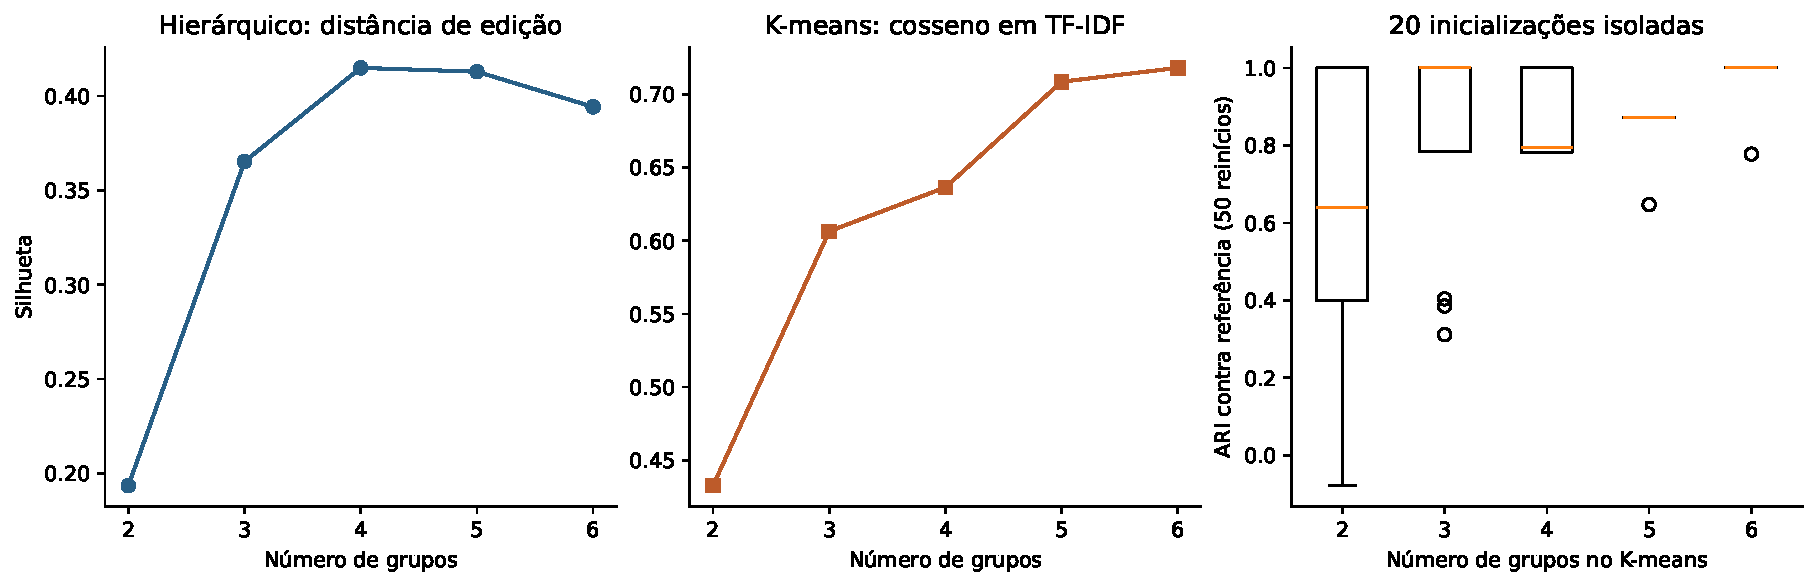
\includegraphics[width=\textwidth]{figures/analysis_diagnostics.pdf}
\caption{Diagnósticos da grade de dois a seis grupos e sensibilidade do K-means à inicialização. As silhuetas são mostradas em painéis separados por utilizarem representações e distâncias distintas; os ARI não expressam incerteza populacional.}\label{fig:diagnostics}
\end{figure}

\begin{figure}[htbp]
\centering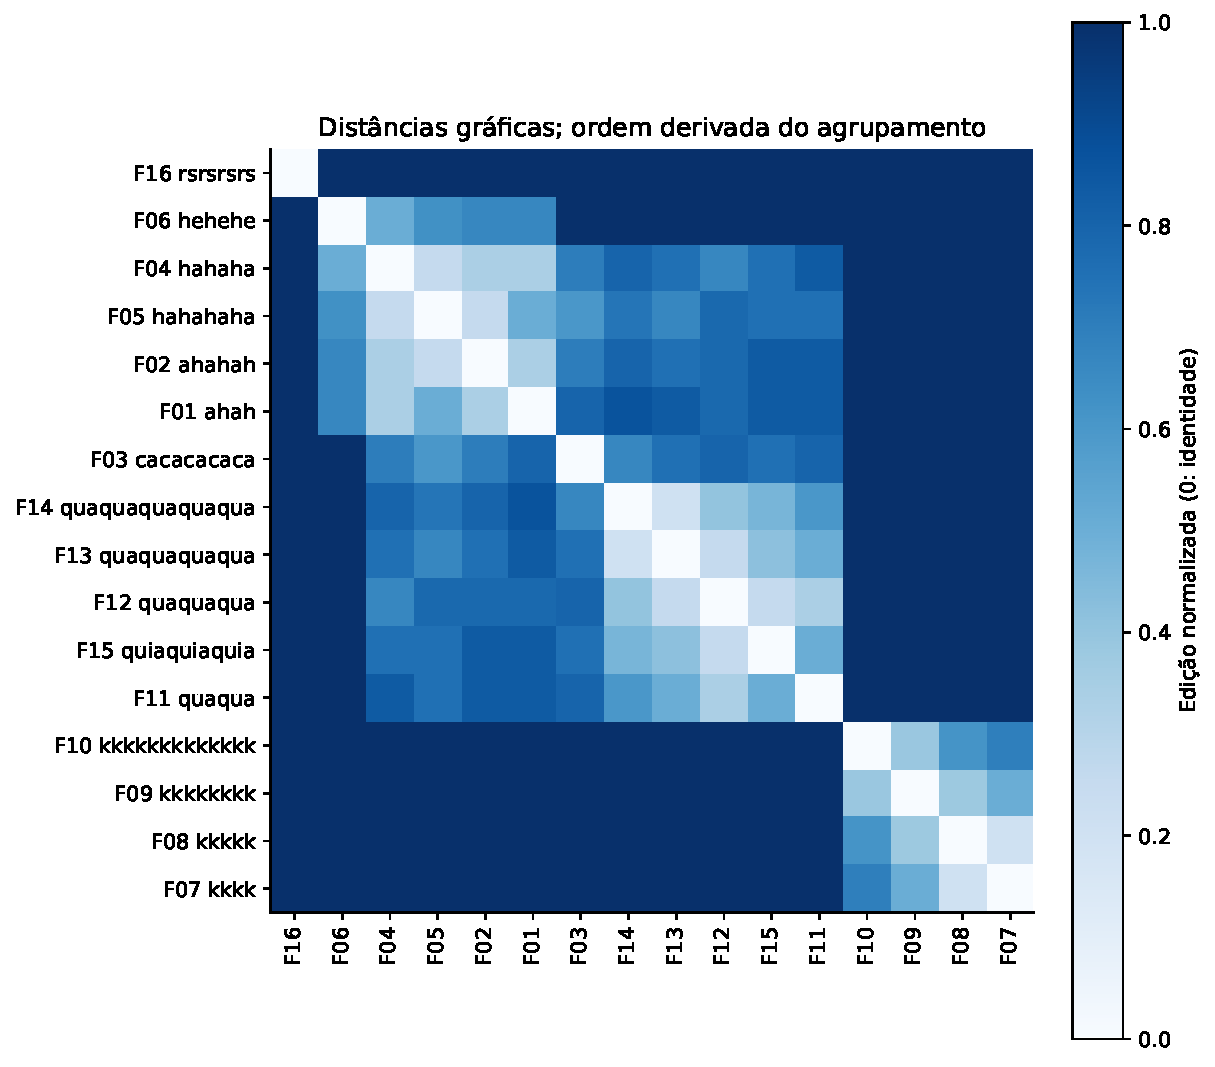
\includegraphics[width=.88\textwidth]{figures/analysis_distances.pdf}
\caption{Matriz de distâncias de edição normalizadas, ordenada pelo agrupamento hierárquico. Os identificadores F01--F16 remetem à Tabela~\ref{tab:form-clusters} e aos arquivos de dados.}\label{fig:distances}
\end{figure}

\small\begin{longtable}{lp{.32\textwidth}rrl}
\caption{Formas normalizadas distintas e partições exploratórias. H: hierárquico com quatro grupos; K: K-means com seis. Datas são extremos selecionados, não origem ou duração de uso.}\label{tab:form-clusters}\\
\toprule ID & Sequência & H & K & Datas selecionadas \\ \midrule\endfirsthead
\toprule ID & Sequência & H & K & Datas selecionadas \\ \midrule\endhead
F01 & \texttt{ahah} & 1 & 3 & 1941--1941 \\
F02 & \texttt{ahahah} & 1 & 3 & 1901--1979 \\
F03 & \texttt{cacacacaca} & 2 & 6 & 1884--1884 \\
F04 & \texttt{hahaha} & 1 & 3 & 2016--2016 \\
F05 & \texttt{hahahaha} & 1 & 3 & 1938--1938 \\
F06 & \texttt{hehehe} & 1 & 5 & 2014--2014 \\
F07 & \texttt{kkkk} & 3 & 1 & 2007--2015 \\
F08 & \texttt{kkkkk} & 3 & 1 & 2022--2022 \\
F09 & \texttt{kkkkkkkk} & 3 & 1 & 2010--2010 \\
F10 & \texttt{kkkkkkkkkkkkk} & 3 & 1 & 2010--2010 \\
F11 & \texttt{quaqua} & 2 & 2 & 1927--1932 \\
F12 & \texttt{quaquaqua} & 2 & 2 & 1919--1956 \\
F13 & \texttt{quaquaquaqua} & 2 & 2 & 1929--1929 \\
F14 & \texttt{quaquaquaquaqua} & 2 & 2 & 2019--2019 \\
F15 & \texttt{quiaquiaquia} & 2 & 2 & 1872--1872 \\
F16 & \texttt{rsrsrsrs} & 4 & 4 & 2010--2010 \\
\bottomrule\end{longtable}\normalsize


\subsection{Reprodução, alcance e limitações específicas}
O script \nolinkurl{scripts/analyze_forms.py} e as dependências em \nolinkurl{requirements-analysis.txt} reconstroem os gráficos e os resultados. O repositório \repo\ publica \href{https://github.com/murilloed/historia-riso-escrito-portugues/blob/main/data/analysis/summary.json}{parâmetros, versões e hash do arquivo de entrada}, vínculos de forma, unidades normalizadas, matriz de distâncias, variáveis TF-IDF, contagens por década e diagnósticos. Os identificadores dos grupos são arbitrários e não são códigos de etapas históricas.

O conjunto de 16 unidades é pequeno, contém formas documentadas de modo desigual e depende de transcrições selecionadas. Não foram estimadas precisão, revocação, acurácia preditiva ou prevalência. A distinção entre registro documental e unidade gráfica evita multiplicar um documento com duas formas, mas não remove vieses de preservação e seleção. A contribuição executada é uma caracterização descritiva e uma comparação exploratória de similaridades gráficas. A demonstração de transmissão histórica continua a exigir documentação de circulação e aprendizagem que as distâncias não fornecem.
\clearpage
